\documentclass[11pt]{article}
\usepackage[T1]{fontenc}
\usepackage[utf8]{inputenc}
% Bera Mono (sans-serif monospaced): sets \ttdefault so \texttt/\ttfamily code
% text matches the project's fixed-width face.
\usepackage[scaled=0.92]{beramono}
\usepackage{amsmath}
\usepackage{amssymb}
\usepackage{mathtools}
\usepackage{geometry}
\usepackage{booktabs}
\usepackage{array}
\usepackage{tabularx}
\usepackage{siunitx}
\usepackage{graphicx}
\usepackage{xcolor}
\usepackage{hyperref}

\geometry{letterpaper, margin=1in}
\graphicspath{{Figs/}}

\hypersetup{
  colorlinks=true,
  linkcolor=blue!60!black,
  urlcolor=blue!60!black,
  citecolor=blue!60!black,
}

% Notation.
\newcommand{\OPD}{\mathrm{OPD}}
\newcommand{\dnupk}{\delta\nu_{\mathrm{pk}}}
\newcommand{\fmod}{f_{\mathrm{mod}}}
\newcommand{\Aphi}{A_{\varphi}}
\newcommand{\Sn}{S_{n}}
\newcommand{\dd}{\mathrm{d}}

% Numeric values and per-case results, auto-generated by make_figures.py.
% Auto-generated by make_figures.py -- do not edit by hand.
% Regenerate with:  make figs   (or  python make_figures.py)
\newcommand{\actuatortf}{376}
\newcommand{\caseAagree}{2.7e-04}
\newcommand{\caseAchone}{45.8}
\newcommand{\caseAchtwo}{46.9}
\newcommand{\caseAcoh}{1.000}
\newcommand{\caseAdrift}{20.0}
\newcommand{\caseAfile}{FM1Day06\_AnchoredAirOPD\_EDUbase\_R1\_20260609\_135823.zip}
\newcommand{\caseAfmod}{100}
\newcommand{\caseAfreqoff}{-0.00}
\newcommand{\caseAharm}{1.29e-02}
\newcommand{\caseAleak}{1.00}
\newcommand{\caseAlockinopd}{1.0717}
\newcommand{\caseAmode}{coherent}
\newcommand{\caseAnoise}{0.41}
\newcommand{\caseAopd}{1.0714}
\newcommand{\caseAopdum}{1071.4}
\newcommand{\caseAshort}{R1, anchored, air}
\newcommand{\caseAsnr}{2611}
\newcommand{\caseAspecopd}{1.0717}
\newcommand{\caseBagree}{3.6e-02}
\newcommand{\caseBchone}{46.2}
\newcommand{\caseBchtwo}{46.1}
\newcommand{\caseBcoh}{0.996}
\newcommand{\caseBdrift}{24.6}
\newcommand{\caseBfile}{FM1Day09\_VacuumReleasedOPD\_SHIMMED\_FLIGHTTORQUED\_R1\_20260629\_140109.zip}
\newcommand{\caseBfmod}{95}
\newcommand{\caseBfreqoff}{+0.48}
\newcommand{\caseBharm}{3.35e-01}
\newcommand{\caseBleak}{1.84}
\newcommand{\caseBlockinopd}{0.1638}
\newcommand{\caseBmode}{coherent}
\newcommand{\caseBnoise}{1.42}
\newcommand{\caseBopd}{0.0892}
\newcommand{\caseBopdum}{89.2}
\newcommand{\caseBshort}{R1, released, vacuum}
\newcommand{\caseBsnr}{63}
\newcommand{\caseBspecopd}{0.0924}
\newcommand{\caseCagree}{5.9e-02}
\newcommand{\caseCchone}{69.5}
\newcommand{\caseCchtwo}{69.3}
\newcommand{\caseCcoh}{0.090}
\newcommand{\caseCdrift}{158.3}
\newcommand{\caseCfile}{FM1Day09\_VacuumReleasedOPD\_SHIMMED\_FLIGHTTORQUED\_R2\_20260629\_140110.zip}
\newcommand{\caseCfmod}{95}
\newcommand{\caseCfreqoff}{-8.52}
\newcommand{\caseCharm}{1.37e-01}
\newcommand{\caseCleak}{1.03}
\newcommand{\caseClockinopd}{0.2789}
\newcommand{\caseCmode}{incoherent}
\newcommand{\caseCnoise}{9.79}
\newcommand{\caseCopd}{0.2713}
\newcommand{\caseCopdum}{271.3}
\newcommand{\caseCshort}{R2, released, vacuum}
\newcommand{\caseCsnr}{28}
\newcommand{\caseCspecopd}{0.2874}
\newcommand{\cmaopd}{45.820}
\newcommand{\cmatone}{2.873e-02}
\newcommand{\cmbopd}{46.892}
\newcommand{\cmbtone}{2.941e-02}
\newcommand{\cmdiffopd}{1.072}
\newcommand{\cmdifftone}{6.721e-04}
\newcommand{\cmrejection}{606}
\newcommand{\cmstda}{4.31}
\newcommand{\cmstdb}{4.31}
\newcommand{\cmstddiff}{0.0071}
\newcommand{\cohthresh}{0.7}
\newcommand{\demodbw}{0.5}
\newcommand{\freqdevpk}{188}
\newcommand{\modvpp}{1.0}


\title{Estimating the residual differential OPD of a dual heterodyne
interferometer from frequency-modulated phasemeter data\\
\large Measurement principle, the leakage-immune demodulation pipeline, and
three test cases from the FM1 campaign}
\author{HET IFO OPD analysis}
\date{\today}

\begin{document}

\maketitle

\begin{abstract}
A known single-tone modulation of the laser frequency turns a heterodyne
interferometer pair into a self-calibrating sensor of its residual optical
path-length difference (OPD): the modulation writes a phase tone on the
differential interferometer phase whose amplitude is proportional to the OPD,
independently of the laser wavelength and of the large, slowly drifting absolute
interferometer phase. This note derives that relation, describes the FM1 unit and
its two dual-interferometer systems, explains why the differential phase is the
right observable (it rejects the common laser frequency noise by
$\sim\!\cmrejection\times$ in this data), and documents the estimation pipeline
implemented in \texttt{het\_ifo\_opd}: a complex-baseband demodulator that is
immune to the spectral leakage which biases a naive lock-in, an automatic
coherent/incoherent integration choice driven by a measured tone coherence, and
a statistically calibrated uncertainty equal to the Cram\'er-Rao bound. We then
put the pipeline to the test on three deliberately different FM1 acquisitions:
one anchored and clean (system R1), and two released acquisitions from the two
systems R1 and R2, one strongly leakage-biased and one genuinely
phase-incoherent. From these we draw out the pitfalls that dominate this
measurement in practice: spectral leakage from the low-frequency wander, real
test-mass motion masquerading as measurement scatter, actuator nonlinearity, and
calibration of the frequency deviation. All numbers and figures in this note are
regenerated from the raw data by \texttt{make\_figures.py} (\texttt{make}).
\end{abstract}

\tableofcontents

\section{Scope: the instrument and the measurement problem}
\label{sec:scope}

\subsection{The FM1 unit and its two dual-interferometer systems}
\label{sec:instrument}

The FM1 unit comprises two nominally identical dual-interferometer systems,
labelled R1 and R2. Each system is a pair of heterodyne interferometers fed by a
common laser: a reference interferometer with static arms, and a measurement
interferometer one of whose arms terminates on a test mass. The two
interferometers of a system have nearly, but not exactly, matched optical path
lengths, so their difference is a small residual differential OPD. Each
interferometer is read out on one phasemeter channel, and the analysis works with
the difference of the two channels.

The test mass can be held in two states. When it is anchored it is clamped so it
cannot move, and the residual differential OPD is static; measuring it well is
then a pure precision problem. When the test mass is released it is free to move,
and its displacement enters the measurement interferometer directly, so the
differential OPD becomes a time-varying, high-precision probe of the forces
acting on the mass. A released acquisition therefore has a differential OPD that
is dynamic by construction, a point that is central to interpreting the results
below.

The acquisition file names encode, in order, the day, the test-mass state
(anchored or released), the medium (air or vacuum), the mounting configuration,
and the system (R1 or R2). Two mounting descriptors appear: whether the unit is
shimmed, and whether flight torque has been applied at its mechanical interface.
Both describe only how the FM1 unit is mounted to its interface and are expected
to have little or no effect on the differential OPD; confirming that expectation
is one aim of the campaign.

\subsection{The measurement problem}
\label{sec:problem}

The difficulty is one of dynamic range. The absolute OPD of each interferometer
is of order tens of millimetres (roughly \num{45} to \SI{70}{\milli\meter}
across these systems), and the laser frequency noise coupling through it drives
the raw per-channel phase through tens of cycles over a \SI{600}{\second}
record. The residual differential OPD is smaller than the absolute OPD by one to
two orders of magnitude, and, for an anchored system, the modulation tone that
encodes it is smaller still: of order $10^{-4}$~cycles, four to five decades
below the raw phase excursion. Extracting it reliably is as much a
signal-processing problem as a physics one.

This note has two purposes. First, to record the measurement principle and the
estimator in enough detail that the numbers can be trusted and reproduced
(Sections~\ref{sec:principle} to~\ref{sec:pipeline}). Second, to exercise the
pipeline on three real acquisitions that span the regimes it must cope with, and
to distil from them the practical pitfalls to avoid when taking these
measurements (Sections~\ref{sec:cases} to~\ref{sec:pitfalls}). The physics and
analysis parameters used throughout are the FM1 defaults of
\texttt{het\_ifo\_opd.config.OPDConfig}.

\section{Measurement principle}
\label{sec:principle}

\subsection{Frequency modulation encodes the OPD}

A two-beam interferometer with optical path-length difference $\OPD$ converts
the instantaneous optical frequency $\nu(t)$ of the laser into an
interferometric phase
\begin{equation}
  \varphi(t) = \nu(t)\,\frac{\OPD}{c} \qquad [\text{cycles}],
  \label{eq:phi}
\end{equation}
equivalently $\varphi=\OPD/\lambda$. Modulating the laser frequency by a small
amount $\delta\nu(t)$ about its mean therefore produces a phase modulation
\begin{equation}
  \delta\varphi(t) = \frac{\OPD}{c}\,\delta\nu(t),
  \label{eq:dphi}
\end{equation}
because $\dd\varphi/\dd\nu=\OPD/c$. The relation is linear: every Fourier
component of $\delta\nu$ maps to the same component of $\delta\varphi$, scaled by
the constant $\OPD/c$. Driving the laser-frequency actuator with a single tone
$\delta\nu(t)=\dnupk\cos(2\pi\fmod t)$ thus imprints a phase tone of amplitude
\begin{equation}
  \Aphi = \frac{\OPD}{c}\,\dnupk
  \qquad\Longrightarrow\qquad
  \boxed{\;\OPD = \frac{\Aphi\,c}{\dnupk}\;}
  \label{eq:opd}
\end{equation}
where the peak (zero-to-peak) frequency deviation follows from the known drive
and actuator gain,
\begin{equation}
  \dnupk = \frac{\dd\nu}{\dd V}\cdot\frac{V_{\mathrm{pp}}}{2}
  = \SI{\actuatortf}{\mega\hertz\per\volt}\times\frac{\SI{\modvpp}{\volt_{pp}}}{2}
  = \SI{\freqdevpk}{\mega\hertz}.
  \label{eq:dnupk}
\end{equation}
Two features make this attractive. It is wavelength independent: the OPD comes
from the frequency modulation alone, and the \SI{1550}{\nano\meter} carrier
enters only as context. And it needs only the amplitude of a single tone, so the
large, slowly drifting DC interferometer phase is irrelevant. The whole problem
reduces to measuring $\Aphi$ at $\fmod$ as accurately as possible.

\subsection{Why the differential phase}
\label{sec:differential}

The reference and measurement interferometers of a system share the same laser,
so each channel is dominated by the laser frequency noise coupling through that
interferometer's own absolute OPD, the tens-of-cycles wander noted in
Section~\ref{sec:problem}. Their difference $\varphi=\varphi_{\mathrm{meas}}-
\varphi_{\mathrm{ref}}$ cancels this common term and leaves the residual
differential OPD, which for a released system carries the test-mass motion.
Figure~\ref{fig:commonmode} shows this for the clean anchored acquisition
(Case~A): the two channels wander by $\sigma\approx\SI{\cmstda}{cyc}$ each, while
the difference has $\sigma_{A-B}\approx\SI{\cmstddiff}{cyc}$, a common-mode
rejection of $\sim\!\cmrejection\times$. The injected tone is common to both
channels as well and is likewise strongly rejected; what survives in the
difference is the tone due to the residual OPD mismatch. Quantifying the tone in
each channel gives absolute OPDs of $\cmaopd$ and $\SI{\cmbopd}{\milli\meter}$
for the two interferometers, versus $\SI{\cmdiffopd}{\milli\meter}$ in the
difference. The package therefore uses the differential phase
$\varphi=\mathrm{ch1}-\mathrm{ch2}$ as the observable and retains the two
absolute OPDs as diagnostics.

\begin{figure}[ht]
  \centering
  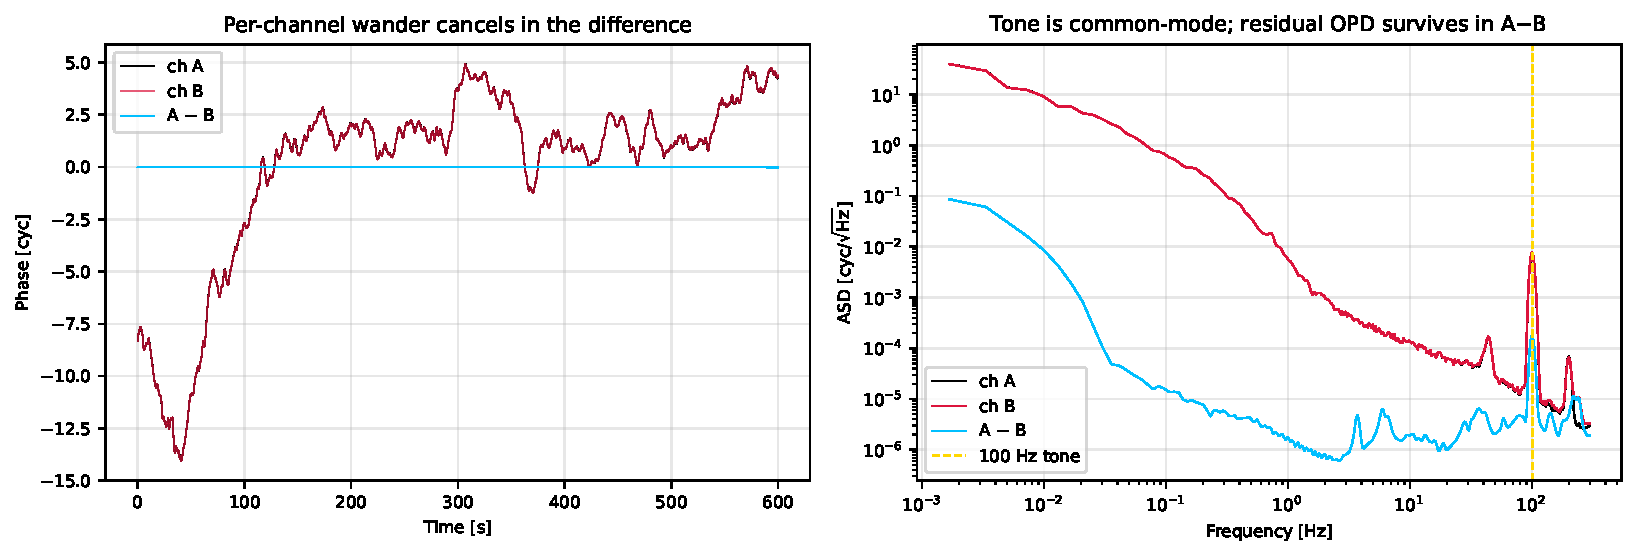
\includegraphics[width=\linewidth]{fig_commonmode.pdf}
  \caption{Common-mode rejection in the clean anchored acquisition (Case~A).
  Left: the two interferometer channels (blue, orange) wander by several cycles,
  driven by laser frequency noise through their absolute OPDs; the difference
  (green) is smaller by $\sim\!\cmrejection\times$. Right: amplitude spectral
  density. The \SI{\caseAfmod}{\hertz} modulation tone (dashed) is large in each
  channel and reduced, but cleanly measurable, in the difference. The
  differential phase is the observable.}
  \label{fig:commonmode}
\end{figure}

\section{The estimation pipeline}
\label{sec:pipeline}

The task of Section~\ref{sec:principle}, measure $\Aphi$ at $\fmod$, looks
elementary but hides a trap that dominated the early analysis. This section
states the trap and the pipeline that removes it. The implementation lives in
\texttt{het\_ifo\_opd.estimators} and \texttt{het\_ifo\_opd.pipeline}.

\subsection{The leakage trap of a naive lock-in}
\label{sec:leakage}

The differential phase is still dominated by a large low-frequency wander
(residual laser-noise coupling, plus real slow test-mass motion on released
systems). A rectangular-window least-squares fit, or a plain DFT, at $\fmod$ has
spectral sidelobes that fall off only as $1/f$, so this enormous out-of-band
content leaks into the $\fmod$ bin and biases the amplitude high. Because the
leakage scales as $\sim\!1/T$, a full-record lock-in can be biased by up to
$\sim\!2\times$ and short per-segment fits by $\sim\!10\times$: this was the
origin of the long-standing puzzle in which the per-segment OPD sat far above the
full-record number. A polynomial detrend and a windowed fit help, but the clean
fix is to isolate a narrow band around the tone before measuring it.

\subsection{Primary estimator: complex-baseband demodulation}
\label{sec:demod}

We heterodyne the tone to DC and low-pass to a narrow one-sided bandwidth $B$:
\begin{equation}
  z(t) = 2\,\mathrm{LPF}_B\!\bigl[\,\varphi(t)\,e^{-2\pi i \fmod t}\,\bigr],
  \qquad |z(t)| = \Aphi(t)\quad[\text{cyc, zero-to-peak}].
  \label{eq:demod}
\end{equation}
The low-pass rejects everything outside $[\fmod-B,\,\fmod+B]$, so the
out-of-band wander physically cannot leak in. This makes $|z(t)|$ the
instantaneous tone amplitude, hence the instantaneous
$\OPD(t)=|z(t)|\,c/\dnupk$, while $\arg z(t)$ is the true tone phase, whose slope
is any residual drive or digitizer frequency offset. The default bandwidth is
$B=\SI{\demodbw}{\hertz}$: wide enough to pass real tone dynamics, narrow enough
to reject the broadband noise and suppress leakage. The FIR low-pass uses a
Kaiser window for a deep, controlled stopband, and the tone frequency is taken
from the known drive and refined on a fine periodogram grid
(\texttt{estimators.refine\_frequency}).

\subsection{Coherent versus incoherent integration}
\label{sec:coherence}

From $z(t)$ we form a coherence
\begin{equation}
  \rho = \frac{|\langle z\rangle|}{\sqrt{\langle|z|^2\rangle}}\in[0,\sim\!1],
  \label{eq:coherence}
\end{equation}
after removing a constant frequency offset, and let it choose how to collapse
$z(t)$ to a single number:
\begin{itemize}
  \item $\rho\ge\cohthresh$ (\texttt{coherence\_threshold}): the tone is
  phase-coherent over the record; report the coherent amplitude
  $|\langle z\rangle|$, the optimal-SNR estimate.
  \item $\rho<\cohthresh$: the tone phase wanders (the OPD is physically moving);
  report the noise-debiased incoherent amplitude
  $\sqrt{\langle|z|^2\rangle-\langle|z_{\mathrm{off}}|^2\rangle}$, the correct
  estimator for a genuinely non-stationary tone, where $z_{\mathrm{off}}$ is an
  off-tone demodulation measuring the in-band noise.
\end{itemize}
This mechanism keeps a moving-test-mass acquisition from being reported as a
falsely precise single value; for such records the instantaneous $\OPD(t)$ is the
real deliverable and the single number is a summary.

\subsection{Uncertainty: noise floor and physical motion}
\label{sec:uncertainty}

Two distinct quantities are reported, and conflating them is itself a pitfall.
The coherent noise floor is the statistical measurement limit,
\begin{equation}
  \sigma_{\Aphi} = \sqrt{\frac{\langle|z_{\mathrm{off}}|^2\rangle}{N_{\mathrm{eff}}}},
  \qquad N_{\mathrm{eff}} = T\cdot 2B,
  \label{eq:sigma}
\end{equation}
with $N_{\mathrm{eff}}$ the number of independent looks. This equals the
Cram\'er-Rao bound $\sqrt{\Sn(\fmod)/T}$ for the local one-sided noise PSD
$\Sn$, and is verified calibrated against Monte-Carlo in the package tests. It
shrinks as $1/\sqrt{T}$ only while the tone is coherent. The physical drift is
the standard deviation of $\OPD(t)$ over the record, a real motion of the test
mass rather than a measurement error, and it does not shrink with $T$. On
anchored records the noise floor dominates and the OPD is a precise number; on
released records the physical motion dominates by orders of magnitude and the OPD
is a moving target, which is exactly the force-sensing signal the released
configuration is built to capture.

\subsection{Cross-checks and quality diagnostics}
\label{sec:diagnostics}

The demodulator is cross-checked and flagged by three further estimators and
ratios, all reported per acquisition:
\begin{itemize}
  \item \texttt{leakage\_ratio} $=A_{\mathrm{lockin}}/A_{\mathrm{demod}}$: the
  rectangular-window lock-in is retained purely as a leakage diagnostic. A value
  near $1$ means the record is clean; a value much greater than $1$ means the
  low-frequency wander is leaking into a naive estimate.
  \item \texttt{method\_agreement} $=|A_{\mathrm{demod}}-A_{\mathrm{spec}}|/
  A_{\mathrm{demod}}$: the demodulator against an independent windowed single-bin
  LPSD estimate (\texttt{speckit}). Both are leakage-suppressed, so a large
  disagreement now flags a real problem, typically incoherence, rather than
  leakage.
  \item \texttt{harmonic\_ratio}: the second-harmonic amplitude relative to the
  fundamental, a live gauge of drive or actuator nonlinearity.
  \item \texttt{tone\_snr} $=A_{\mathrm{demod}}/\sigma_{\Aphi}$: the coherent
  amplitude signal-to-noise ratio.
\end{itemize}

\section{Three test cases}
\label{sec:cases}

We now run the pipeline on three FM1 acquisitions chosen to span its operating
regimes. All three use the FM1 physics defaults; the two Day09 records use
$\fmod=\SI{95}{\hertz}$ and the Day06 record $\SI{100}{\hertz}$. Cases~A and~B
are the same system (R1), anchored and released respectively; Case~C is the other
system (R2) under the same released conditions as Case~B. Both released cases are
shimmed and flight-torqued in vacuum. Table~\ref{tab:cases} collects the headline
results and diagnostics.

\begin{table}[ht]
\centering
\small
\begin{tabularx}{\linewidth}{@{}l >{\raggedright\arraybackslash}X r r r l r r r@{}}
\toprule
\textbf{Case} & \textbf{Configuration} & \textbf{OPD} & \textbf{noise} &
\textbf{drift} & \textbf{mode} & $\boldsymbol{\rho}$ & \textbf{leak} &
\textbf{SNR}\\
 & & [mm] & [\si{\micro\meter}] & [\si{\micro\meter}] & & & $\times$ & \\
\midrule
A & R1, anchored, air        & \caseAopd & \caseAnoise & \caseAdrift & \caseAmode   & \caseAcoh & \caseAleak & \caseAsnr\\
B & R1, released, vacuum      & \caseBopd & \caseBnoise & \caseBdrift & \caseBmode   & \caseBcoh & \caseBleak & \caseBsnr\\
C & R2, released, vacuum      & \caseCopd & \caseCnoise & \caseCdrift & \caseCmode   & \caseCcoh & \caseCleak & \caseCsnr\\
\bottomrule
\end{tabularx}
\caption{Headline results for the three test cases. Case~A is the clean, anchored
reference. Case~B is coherent but strongly leakage-biased (the naive lock-in
over-reads by $\times\caseBleak$). Case~C is genuinely phase-incoherent
($\rho=\caseCcoh$), motion-limited, and correctly reported with the incoherent
estimator. ``noise'' is the coherent noise floor (Eq.~\ref{eq:sigma}); ``drift''
is the standard deviation of $\OPD(t)$.\label{tab:cases}}
\end{table}

\subsection{Case A: clean anchored reference}
\label{sec:caseA}

\texttt{\caseAfile}. This is system R1 with its test mass anchored, the
best-behaved regime and the calibration point for reading the diagnostics. The
tone sits far above the noise (SNR $\approx\caseAsnr$), the demodulator, the
windowed single-bin and even the rectangular lock-in all agree
(\texttt{leakage\_ratio} $=\caseAleak$, \texttt{method\_agreement}
$=\caseAagree$), and the tone is fully coherent ($\rho=\caseAcoh$, mode
\texttt{\caseAmode}). The residual OPD is $\SI{\caseAopd}{\milli\meter}$ with a
coherent noise floor of only $\SI{\caseAnoise}{\micro\meter}$; the
$\SI{\caseAdrift}{\micro\meter}$ of drift in $\OPD(t)$ is small residual motion,
not a limitation. The second-harmonic content is modest (\texttt{harmonic\_ratio}
$=\caseAharm$). Figure~\ref{fig:caseA} shows the three-panel diagnostic: the ASD
with the tone marked, the phase-folded (synchronous-averaged) tone, and the flat
$\OPD(t)$.

\begin{figure}[ht]
  \centering
  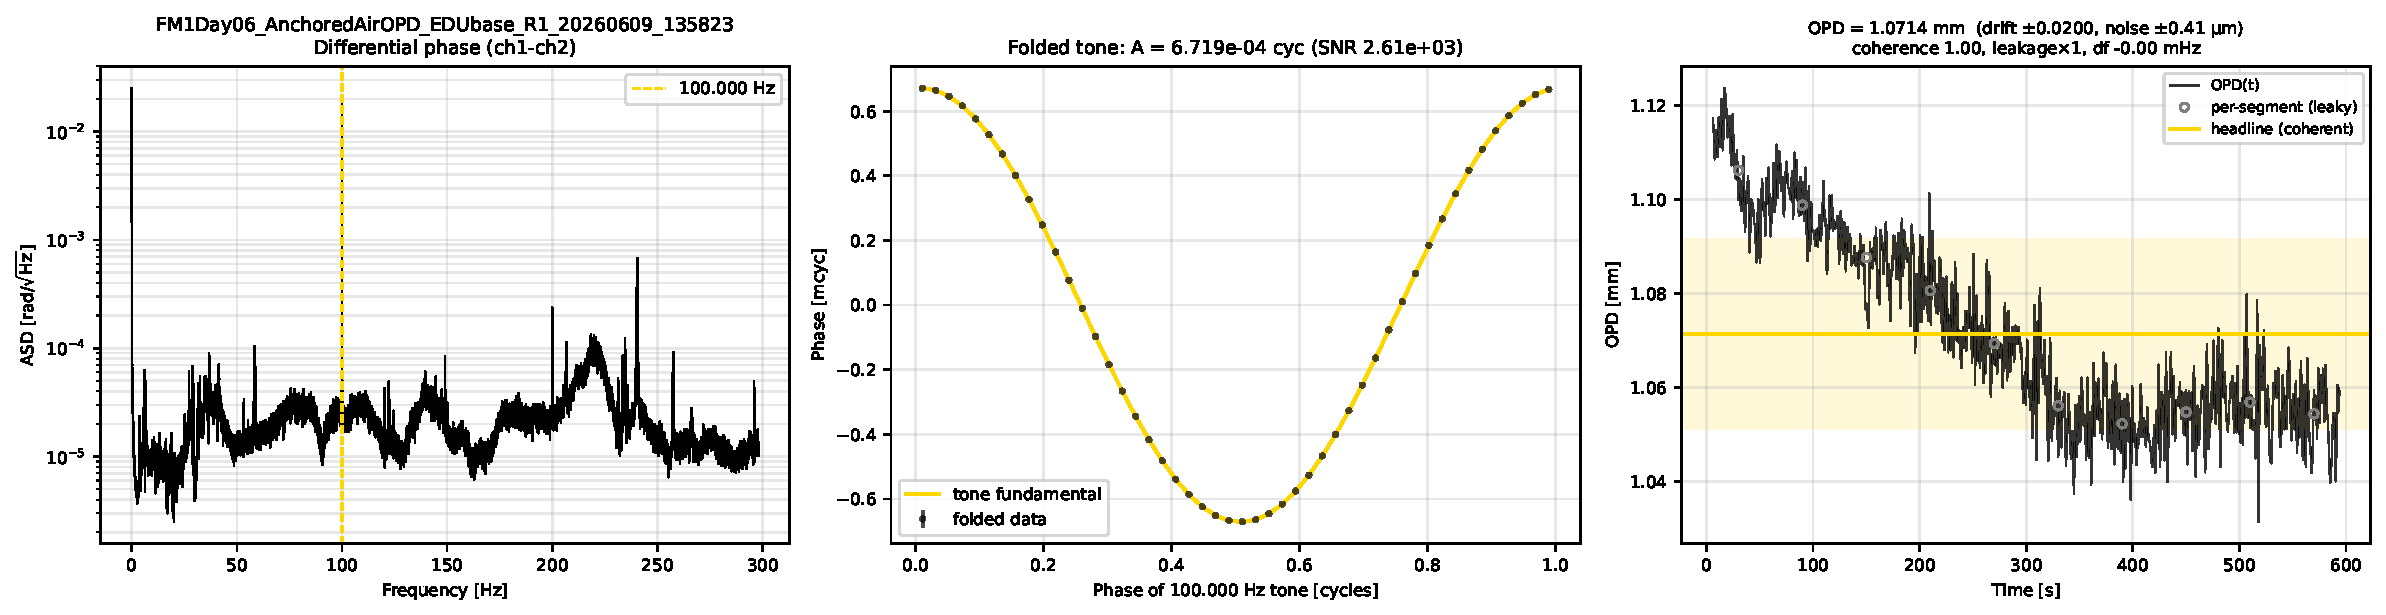
\includegraphics[width=\linewidth]{fig_caseA_diag.pdf}
  \caption{Case~A diagnostics (R1, anchored, air). Left: differential-phase ASD,
  tone at \SI{\caseAfmod}{\hertz} marked. Centre: the phase-folded tone stands
  cleanly above the noise. Right: $\OPD(t)$ is essentially flat; the headline,
  drift band, and (here coincident) per-segment estimates all agree. This is the
  regime in which the frequency-modulation method delivers a precise static OPD.}
  \label{fig:caseA}
\end{figure}

\subsection{Case B: released, coherent but leakage-biased}
\label{sec:caseB}

\texttt{\caseBfile}. This is the same system R1 as Case~A, now with the test mass
released and the unit shimmed and flight-torqued in vacuum. Over this particular
record the tone remains phase-coherent ($\rho=\caseBcoh$, mode
\texttt{\caseBmode}), and the demodulator returns a well-defined
$\SI{\caseBopd}{\milli\meter}$. But the low-frequency wander is now large enough
that a naive rectangular lock-in over-reads by $\times\caseBleak$ (it would report
$\SI{\caseBlockinopd}{\milli\meter}$), while the leakage-immune demodulator and
the windowed single-bin agree far better (\texttt{method\_agreement}
$=\caseBagree$; single-bin $\SI{\caseBspecopd}{\milli\meter}$). This is the
textbook leakage case of Section~\ref{sec:leakage}, caught by
\texttt{leakage\_ratio}. Note also the large second harmonic
(\texttt{harmonic\_ratio} $=\caseBharm$): under torque the drive or actuator
chain is visibly nonlinear, a point we return to in Section~\ref{sec:pitfalls}.
Because the demodulator reads only the fundamental in a narrow band, that
distortion does not corrupt the OPD, but it is a warning flag.
Figure~\ref{fig:caseB} shows the diagnostic; the leakage is visible as the
per-segment markers sitting above the demodulated $\OPD(t)$.

\begin{figure}[ht]
  \centering
  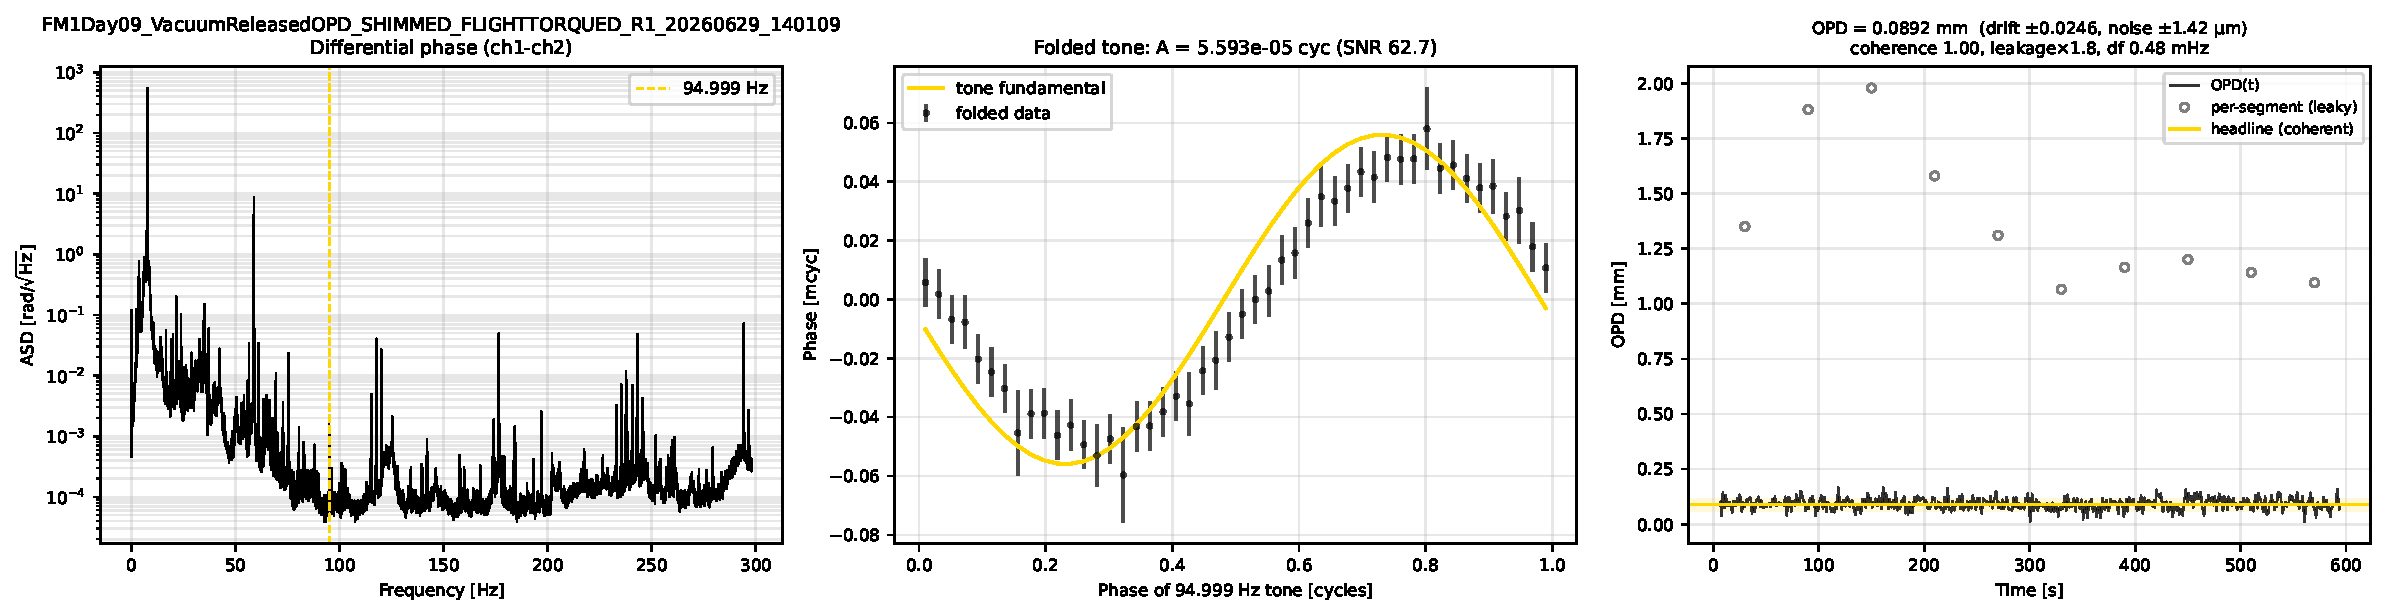
\includegraphics[width=\linewidth]{fig_caseB_diag.pdf}
  \caption{Case~B diagnostics (R1, released, vacuum). The tone is coherent, so
  $\OPD(t)$ is a well-defined $\SI{\caseBopd}{\milli\meter}$, but the
  low-frequency wander biases the rectangular per-segment estimates (grey open
  markers) high, the same leakage that inflates the naive lock-in by
  $\times\caseBleak$. The demodulator is immune to it.}
  \label{fig:caseB}
\end{figure}

\subsection{Case C: released, phase-incoherent (motion-limited)}
\label{sec:caseC}

\texttt{\caseCfile}. This is the other system, R2, under the same released,
shimmed, flight-torqued, vacuum conditions as Case~B, and it behaves very
differently. The test mass is moving over the record, so the tone is not
phase-coherent ($\rho=\caseCcoh$, well below $\cohthresh$) and the pipeline
correctly falls back to the incoherent estimator (mode \texttt{\caseCmode}). The
reported OPD is $\SI{\caseCopd}{\milli\meter}$, but the meaningful quantity here
is the motion: the drift of $\OPD(t)$ is $\SI{\caseCdrift}{\micro\meter}$, more
than an order of magnitude above the $\SI{\caseCnoise}{\micro\meter}$ noise floor.
The leakage ratio is now near unity (\texttt{leakage\_ratio} $=\caseCleak$), so
this record is not leakage-biased, yet \texttt{method\_agreement} is
comparatively poor (\caseCagree), the expected signature of a genuinely
non-stationary tone rather than of leakage. That the two systems have different
absolute OPDs (about $\SI{\caseBchone}{\milli\meter}$ for R1 in Case~B versus
$\SI{\caseCchone}{\milli\meter}$ for R2 here) confirms they are distinct setups,
not repeats. Figure~\ref{fig:caseC} shows the wandering $\OPD(t)$: here the time
series and its statistics, not a single value, are the deliverable.

\begin{figure}[ht]
  \centering
  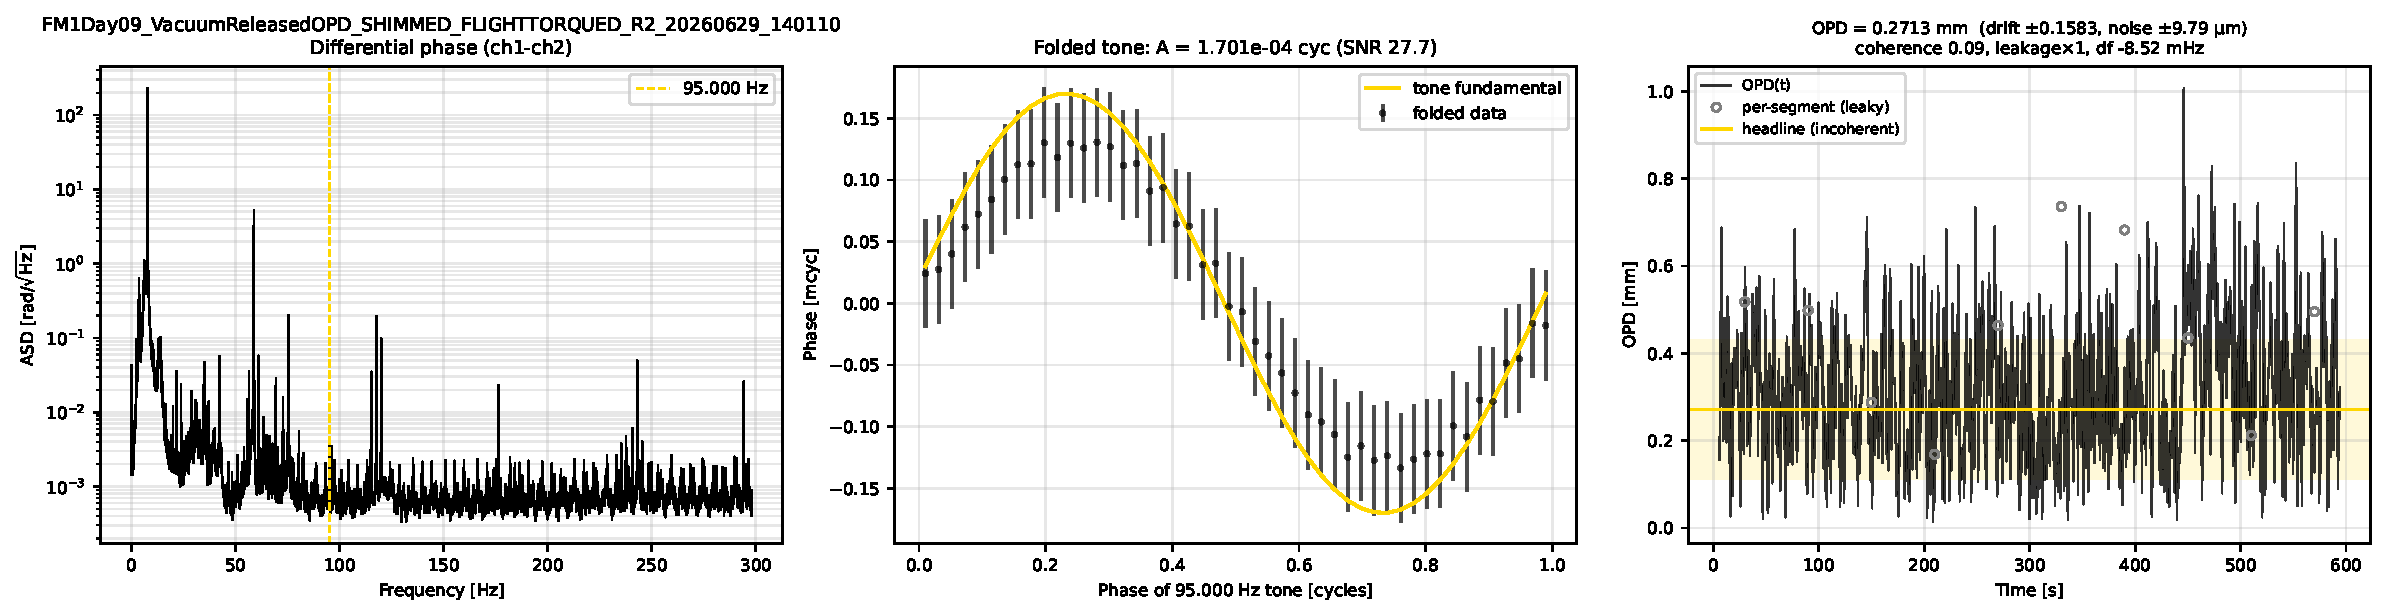
\includegraphics[width=\linewidth]{fig_caseC_diag.pdf}
  \caption{Case~C diagnostics (R2, released, vacuum). $\OPD(t)$ moves by
  $\sim\!\SI{\caseCdrift}{\micro\meter}$ across the record; the tone loses phase
  coherence ($\rho=\caseCcoh$), so the incoherent estimator is used. For a
  released test mass this motion is the science signal, and the deliverable is
  the time series and its statistics, not a single precise value.}
  \label{fig:caseC}
\end{figure}

\subsection{Cross-case comparison}
\label{sec:compare}

Figures~\ref{fig:leakage} and~\ref{fig:opdt} summarise the three cases side by
side. Figure~\ref{fig:leakage} plots the three amplitude estimators as OPDs: for
the clean Case~A they coincide, for Case~B the rectangular lock-in stands well
above the two leakage-immune estimators, and for Case~C all three are close (no
leakage) even though the record is the least meaningful as a single number.
Figure~\ref{fig:opdt} overlays the instantaneous $\OPD(t)$: flat and static (A),
offset but stable over this record (B), and wandering with the released test mass
(C). Two lessons stand out. First, the comparison of Cases~A and~B, the same
system R1 anchored then released, shows how anchoring produces a static,
precisely measurable OPD while releasing introduces both real motion and the
low-frequency wander that leakage feeds on. Second, the comparison of Cases~B
and~C, two different systems under identical conditions, shows that
\texttt{leakage\_ratio} and $\rho$ are independent diagnostics: a record can fail
either test on its own.

\begin{figure}[ht]
  \centering
  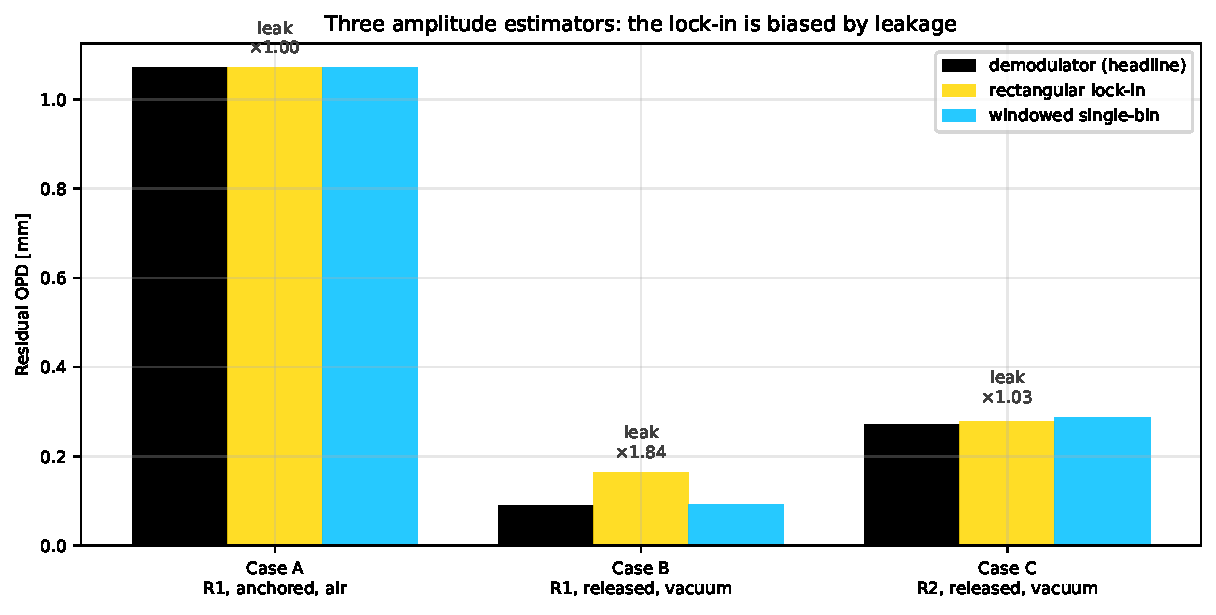
\includegraphics[width=0.86\linewidth]{fig_leakage.pdf}
  \caption{The three amplitude estimators, expressed as OPD, for each case. They
  agree when the record is clean (A), diverge when leakage is present (B, the
  lock-in over-reads by $\times\caseBleak$), and agree again when the problem is
  motion rather than leakage (C). The rectangular lock-in is kept only as this
  diagnostic.}
  \label{fig:leakage}
\end{figure}

\begin{figure}[ht]
  \centering
  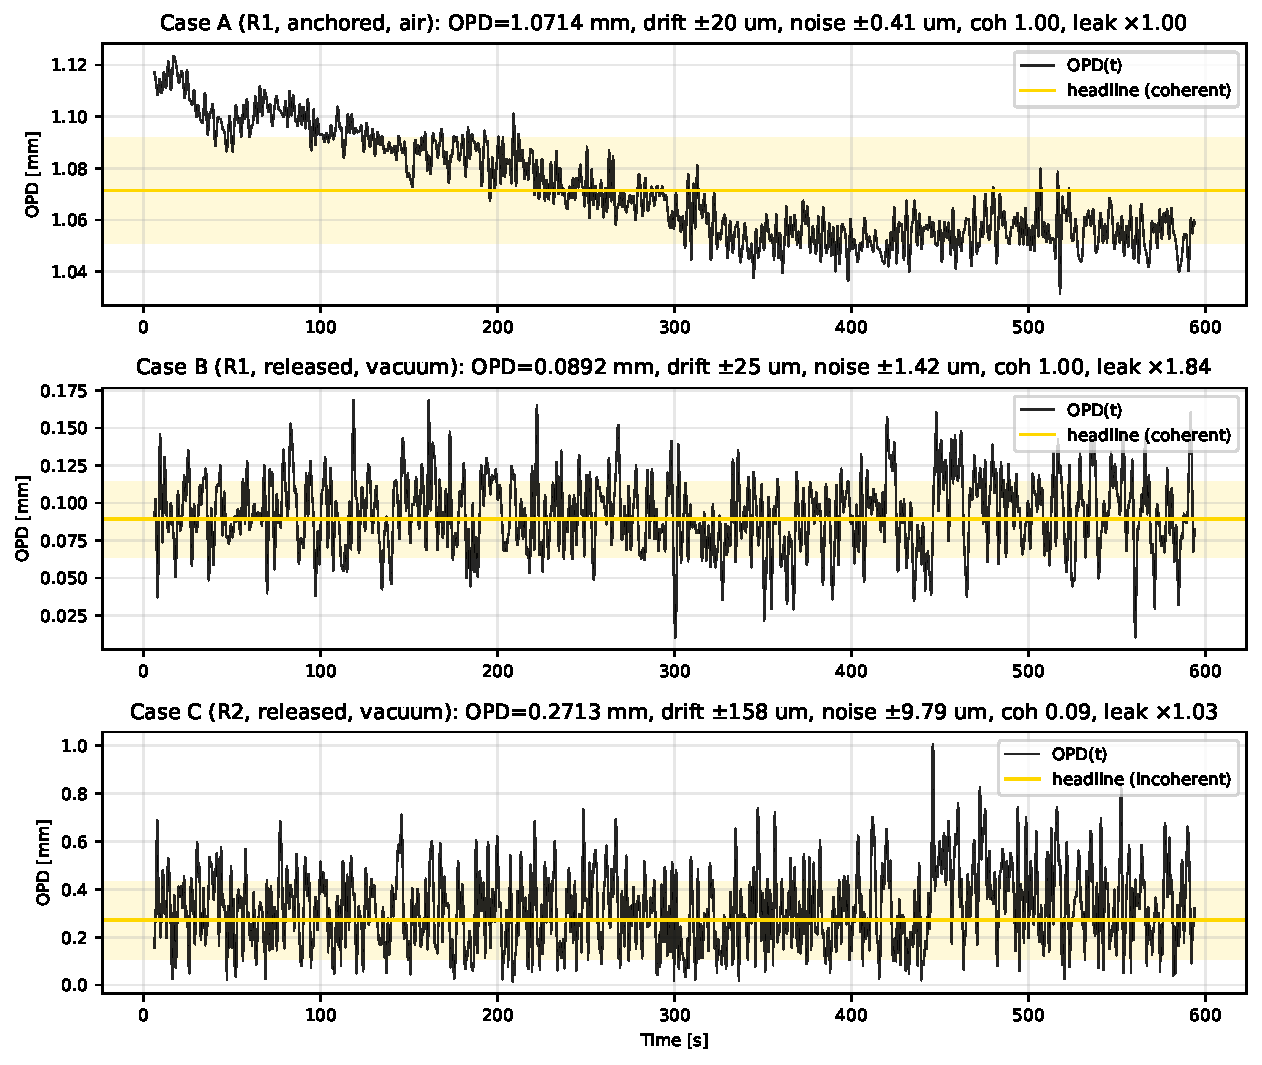
\includegraphics[width=0.86\linewidth]{fig_opd_t.pdf}
  \caption{Instantaneous $\OPD(t)$ from the demodulator for the three cases (note
  the differing vertical scales). Case~A is flat and precise; Case~B is stable
  over this record but offset (and, before correction, leakage-biased); Case~C
  physically wanders with the released test mass and is reported as a time series
  plus its motion statistics.}
  \label{fig:opdt}
\end{figure}

\section{Pitfalls to avoid}
\label{sec:pitfalls}

The three cases, together with the wider FM1 set, make the recurring failure
modes concrete. We list them roughly in order of how often they bite.

\paragraph{1. Spectral leakage from the low-frequency wander (Case~B).}
A rectangular-window lock-in or plain DFT at $\fmod$ leaks the tens-of-cycles
low-frequency content into the tone bin and over-reports the OPD, by up to
$\sim\!2\times$ on a full record and up to $\sim\!10\times$ on short segments.
This is the single most damaging analysis error, and it is entirely avoidable:
demodulate in a narrow band (Section~\ref{sec:demod}) and treat any
\texttt{leakage\_ratio} much greater than $1$ as a red flag. Do not quote
short-segment rectangular estimates as the OPD.

\paragraph{2. Confusing real motion with measurement precision (Case~C).}
When the test mass is released the OPD is time-varying by construction, so the
coherent noise floor (Eq.~\ref{eq:sigma}) is not the uncertainty on ``the'' OPD;
there is no single OPD. Reporting $\SI{\caseCnoise}{\micro\meter}$ for Case~C
would be off by more than an order of magnitude from the
$\SI{\caseCdrift}{\micro\meter}$ of real motion. Watch the \texttt{mode} and
$\rho$ flags: a low coherence means report $\OPD(t)$ and its statistics, not a
precise number. Longer records do not shrink the motion; they only characterise
it better.

\paragraph{3. A released test mass has no single OPD.}
Following from the previous point: to obtain one static differential-OPD value
the test mass must be anchored (Cases~A). A released system is designed to let
the mass move, and the demodulated $\OPD(t)$ is then the force-sensing signal. Do
not force a single number onto a released record; report the trajectory.

\paragraph{4. Actuator or drive nonlinearity.}
The torqued Case~B shows a large second harmonic (\texttt{harmonic\_ratio}
$=\caseBharm$, against $\caseAharm$ for the clean Case~A). Harmonics themselves do
not corrupt the OPD, since only the fundamental is read, but they signal that the
actuator may be compressing the fundamental, which biases the calibration
$\dnupk=(\dd\nu/\dd V)V_{\mathrm{pp}}/2$ low. Push the modulation amplitude up for
SNR, but monitor \texttt{harmonic\_ratio}, back off if it rises sharply, and
calibrate $\dnupk$ at the actual operating depth rather than trusting the
small-signal $\dd\nu/\dd V$.

\paragraph{5. Calibration of the frequency deviation.}
$\dnupk$ is a direct multiplicative scale on the OPD (Eq.~\ref{eq:opd}), yet it is
currently assumed from a nominal $\dd\nu/\dd V=\SI{\actuatortf}{\mega\hertz\per\volt}$
taken as flat. Any error in $\dd\nu/\dd V$, in its frequency dependence at
$\fmod$, or in the actually delivered $V_{\mathrm{pp}}$ maps one-to-one onto the
OPD. This is the leading accuracy systematic and deserves a dedicated in-situ
calibration.

\paragraph{6. Modulation-frequency choice and clocking.}
Place $\fmod$ in a quiet valley of the differential-phase noise, away from line
harmonics and mechanical resonances, and keep it and its first few harmonics
comfortably below Nyquist. Share a common clock between the drive source and the
phasemeter: an unshared clock leaves a residual tone-frequency offset (for
example $\SI{\caseCfreqoff}{\milli\hertz}$ for Case~C) that the pipeline must fit
out and that can erode coherence over long records.

\section{Summary and recommendations}
\label{sec:summary}

A known single-tone laser-frequency modulation turns each interferometer pair
into a self-calibrating OPD sensor: the residual OPD is $\OPD=\Aphi c/\dnupk$,
read from the amplitude of the tone in the differential phase, wavelength
independent and immune to the large DC interferometer phase. The estimation
pipeline is a complex-baseband demodulator that is immune to the spectral leakage
which biased the naive lock-in, yields the instantaneous $\OPD(t)$, chooses
coherent versus incoherent integration from a measured coherence, and reports an
uncertainty equal to the Cram\'er-Rao bound. Applied to three FM1 acquisitions it
recovers a sub-micron-precise $\SI{\caseAopd}{\milli\meter}$ on the clean anchored
record (R1), correctly de-biases the leaky released record (R1) from
$\SI{\caseBlockinopd}{\milli\meter}$ (lock-in) to $\SI{\caseBopd}{\milli\meter}$,
and correctly reports the incoherent released record (R2) as a moving $\OPD(t)$
rather than a false precise value.

For the experimentalist, the levers that most improve a static differential-OPD
measurement are, in order: anchor and mechanically quiet the interferometer (this
gives a well-defined static OPD and enables long coherent integration); increase
the modulation amplitude for SNR while monitoring the second harmonic
(pitfall~4); calibrate $\dnupk$ in situ (pitfall~5); choose $\fmod$ in a noise
valley with a shared clock (pitfall~6). For the analyst, the rules are: never
quote a rectangular short-segment amplitude as the OPD (pitfall~1), and always
read the \texttt{leakage\_ratio}, coherence and \texttt{mode}, and
\texttt{method\_agreement} flags before trusting a single number. When coherence
is low the mass is moving, so report the $\OPD(t)$ time series and its statistics
instead.

\section*{Reproducibility}
\addcontentsline{toc}{section}{Reproducibility}

Every number and figure in this note is produced from the raw FM1 files by
\texttt{make\_figures.py}, which runs \texttt{het\_ifo\_opd.pipeline.estimate\_opd}
on the three cases, writes the figures to \texttt{Figs/}, and emits the numeric
macros in \texttt{values.tex}. Rebuild the whole note with \texttt{make} (which
runs the script and then \texttt{pdflatex}), or regenerate only the figures and
values with \texttt{make figs}.

\section*{References}
\addcontentsline{toc}{section}{References}

\begin{sloppypar}
\begin{itemize}
  \item Package and pipeline: \texttt{het\_ifo\_opd} (\texttt{estimators.py},
        \texttt{pipeline.py}, \texttt{physics.py}, \texttt{config.py}); the
        end-to-end walk-through in
        \texttt{notebooks/fm1\_opd\_analysis.ipynb}; project \texttt{README.md}.
  \item Estimator validation (leakage-immunity, calibrated uncertainty near the
        Cram\'er-Rao bound, incoherent fallback): \texttt{tests/}.
  \item Spectral tooling: \texttt{speckit} (LPSD single-bin and windowed ASD);
        Moku:Pro Phasemeter I/O: \texttt{mokutools}.
\end{itemize}
\end{sloppypar}

\end{document}
